\documentclass[12pt,a4paper]{article}

% ========== 基础宏包 ==========
\usepackage{ctex}
\usepackage{graphicx}
\usepackage{amsmath,amssymb}
\usepackage{geometry}
\usepackage{fancyhdr}
\usepackage{booktabs}
\usepackage{multirow}
\usepackage{setspace}
\usepackage{array}
\usepackage{lastpage}
\usepackage{caption}
\usepackage{enumitem}
\usepackage{float}
\usepackage{xcolor}
\usepackage{adjustbox}

% ========== 页面设置 ==========
\geometry{
    left=2.5cm,
    right=2.5cm,
    top=2.5cm,
    bottom=2.5cm,
    headheight=15pt
}

% ========== 页眉页脚 ==========
\pagestyle{fancy}
\fancyhf{}
\fancyhead[C]{\small 哈尔滨工业大学（深圳）实验报告}
\fancyfoot[C]{\thepage\,/\,\pageref{LastPage}}
\renewcommand{\headrulewidth}{0.4pt}

% ========== 标题表格设置 ==========
\captionsetup{font=small,labelfont=bf,skip=0.5em}
\renewcommand{\arraystretch}{1.3}

% ========== 列表 ==========
\setlist[enumerate]{leftmargin=2em, itemsep=0.3em}
\setlist[itemize]{leftmargin=2em, itemsep=0.2em}

% ========== 段落 ==========
\setlength{\parindent}{2em}
\setlength{\parskip}{0.5em}

% ========== 封面命令（真正居中、不溢出）==========
\newcommand{\coverline}[1]{%
    \raisebox{-4pt}{\underline{\makebox[10.5cm][c]{#1}}}%
}

\begin{document}

% ===================== 封面（完美版）=====================
\begin{titlepage}
    \centering
    \vspace*{2cm}

    {\zihao{2}\heiti 哈尔滨工业大学（深圳）}\\[0.6em]
    {\zihao{4} Harbin Institute of Technology, Shenzhen}\\[3em]

    {\zihao{1}\heiti 实\quad 验\quad 报\quad 告}\\[4em]

    \begin{tabular}{ll}
        \heiti\zihao{4} 课程名称： & \coverline{自动控制理论} \\[0.8em]
        \heiti\zihao{4} 学生姓名： & \coverline{余泓彬} \\[0.8em]
        \heiti\zihao{4} 班级学号： & \coverline{2024312506} \\[0.8em]
        \heiti\zihao{4} 学生专业： & \coverline{电气类} \\[0.8em]
        \heiti\zihao{4} 实验名称： & \coverline{实验三 线性系统的频率响应实验} \\[0.8em]
        \heiti\zihao{4} 报告时间： & \coverline{2026-05-15} \\
    \end{tabular}

    \vfill
    {\zihao{4}\heiti 哈尔滨工业大学（深圳）}\\[1em]
\end{titlepage}

% ===================== 正文 =====================
\section{实验目的}
\begin{enumerate}
    \item 掌握测量典型一阶、二阶系统频率特性曲线的实验方法，理解频率响应的基本概念。
    \item 了解频率特性的测试原理，通过实验进一步理解频率特性的物理意义。
    \item 学会绘制一阶、二阶线性系统的对数幅频特性曲线和相频特性曲线（Bode图）。
    \item 通过实验验证理论分析结果，加深对频率响应分析方法的理解，掌握利用Bode图分析系统性能的方法。
    \item 观察阻尼比、增益等参数对二阶系统频率特性的影响，理解不同阻尼比下系统幅频和相频特性的变化规律。
\end{enumerate}

\section{实验设备及元器件}
\begin{itemize}
    \item PC机一台（安装有LabVIEW实验软件）
    \item NI ELVIS III实验平台一台
    \item ``Circuits Control Board - 1''（自动控制原理课程实验套件1）
    \item 导线若干（本实验需3根）
\end{itemize}

\section{实验原理及实验过程}

\subsection{实验原理}

\subsubsection{频率特性的基本概念}
当输入正弦信号时，线性系统的稳态响应具有随频率 $\omega$（由 $0$ 变至 $\infty$）而变化的特性。频率响应法的基本思想是：实际输入的周期信号都能满足狄利克莱条件，可以用傅里叶级数展开为各种谐波分量；而非周期信号也可以使用傅里叶积分表示为连续的频谱函数。因此，根据控制系统对正弦输入信号的响应，可推算出系统在任意周期信号或非周期信号作用下的运动情况。

\subsubsection{线性系统的频率特性}
系统的正弦稳态响应具有和正弦输入信号的幅值比 $|\Phi(\mathrm{j}\omega)|$ 和相位差 $\angle\Phi(\mathrm{j}\omega)$ 随频率 $\omega$（由 $0$ 变至 $\infty$）变化的特性。而幅值比 $|\Phi(\mathrm{j}\omega)|$ 和相位差 $\angle\Phi(\mathrm{j}\omega)$ 恰好是函数 $\Phi(\mathrm{j}\omega)$ 的模和幅角。所以只要在系统的传递函数 $\Phi(s)$ 中，令 $s=\mathrm{j}\omega$，即可得到 $\Phi(\mathrm{j}\omega)$。我们把 $\Phi(\mathrm{j}\omega)$ 称为系统的频率特性或频率传递函数。当 $\omega$ 由 $0$ 到 $\infty$ 变化时，$|\Phi(\mathrm{j}\omega)|$ 随频率 $\omega$ 的变化特性成为幅频特性，$\angle\Phi(\mathrm{j}\omega)$ 随频率 $\omega$ 的变化特性称为相频特性。幅频特性和相频特性结合在一起时称为频率特性。

\subsubsection{对数频率特性（波特图）}
对数频率特性，又称波特图，它包括对数幅频和对数相频两条曲线，是频率响应法中广泛使用的一组曲线。这两组曲线连同它们的坐标组成了对数坐标图。对数频率特性图的优点有：
\begin{itemize}
    \item 它把各串联环节幅值的乘除化为加减运算，从而简化了开环频率特性的计算与作图。
    \item 利用渐近直线来绘制近似的对数幅频特性曲线，而且对数相频特性曲线具有奇对称于转折频率点的性质，这些可使作图大为简化。
    \item 通过对数的表达式，可以在一张图中既能绘制出频率特性的中、高频特性，又能清晰地画出其低频特性。
\end{itemize}
本次实验中，采用对数频率特性图来进行频域响应分析。

\subsection{一阶惯性环节}
\subsubsection{方框图与模拟电路图}
\begin{figure}[H]
    \centering
    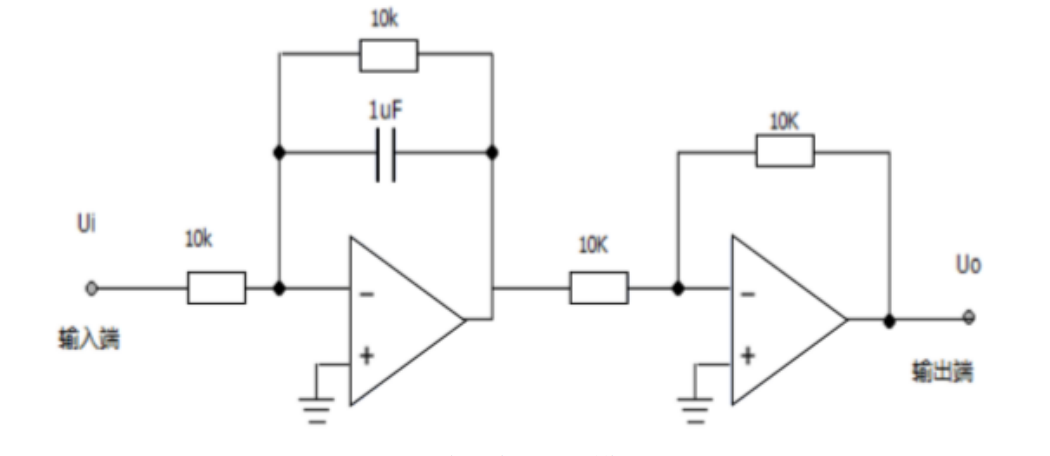
\includegraphics[width=0.8\textwidth]{3.1.png}
    \caption{一阶惯性环节模拟电路图}
    \label{fig:circuit1}
\end{figure}

\subsubsection{一阶系统实测幅频特性图}
\begin{figure}[H]
    \centering
    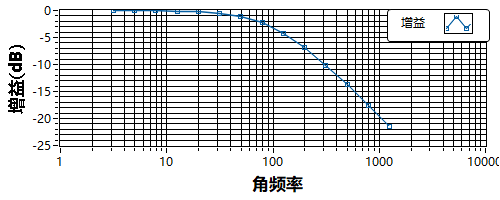
\includegraphics[width=0.8\textwidth]{1.1.png}
    \caption{一阶惯性环节实测幅频增益特性曲线}
\end{figure}

\subsubsection{一阶系统实测相频特性图}
\begin{figure}[H]
    \centering
    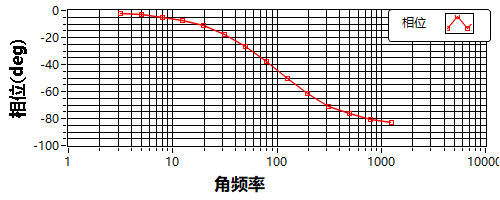
\includegraphics[width=0.8\textwidth]{1.2.png}
    \caption{一阶惯性环节实测相频相位特性曲线}
\end{figure}

\subsubsection{传递函数推导}
一阶惯性环节的传递函数为：
\begin{equation}
G(s) = \frac{1}{1+Ts}
\end{equation}
其频率特性为：
\begin{equation}
G(\mathrm{j}\omega) = \frac{1}{1+\mathrm{j}\omega T}
\end{equation}
对数幅频特性：
\begin{equation}
L(\omega) = -20\lg\sqrt{1+(\omega T)^2}
\end{equation}
相频特性：
\begin{equation}
\varphi(\omega) = -\arctan(\omega T)
\end{equation}
其中 $T=0.01\,\mathrm{s}$。

\paragraph{实验步骤}
\begin{enumerate}
    \item 计算一阶惯性环节在不同频率下的幅值和相位，填入表\ref{tab:first-order}，并与实验测得曲线作比较，分析实验数值和理论数值是否匹配。
    \item 通过实测曲线，观察一阶惯性系统截止频率和相位，附上图形及数据。
\end{enumerate}

\subsubsection{一阶惯性环节幅频和相频理论与实测结果对比}
\begin{table}[H]
\centering
\caption{一阶惯性环节幅频和相频理论与实测结果对比}
\label{tab:first-order}
\adjustbox{max width=\linewidth}{
\begin{tabular}{|c|c|c|c|c|c|}
\hline
\multirow{2}{*}{\textbf{计算公式}} & $\omega$ & $L(\omega)$ 计算 & $\varphi(\omega)$ 计算 & $L(\omega)$ 实测 & $\varphi(\omega)$ 实测 \\
\cline{2-6}
 & (rad/s) & (dB) & (deg) & (dB) & (deg) \\
\hline
\multirow{3}{*}{
\parbox{3.8cm}{\centering
$L=-20\lg\sqrt{1+T^2\omega^2}$\\
$\varphi=-\arctan(T\omega)$\\
$T=0.01\,\mathrm{s}$
}}
 & 10   & -0.04  & -5.71  & -0.042 & -2.05 \\
\cline{2-6}
 & 100  & -3.01  & -45.00 & -3.01  & -45.00 \\
\cline{2-6}
 & 1000 & -20.04 & -84.29 & -21.39 & -83.11 \\
\hline
\end{tabular}
}
\end{table}

\subsection{二阶线性系统}
\subsubsection{方框图与模拟电路图}
\begin{figure}[H]
    \centering
    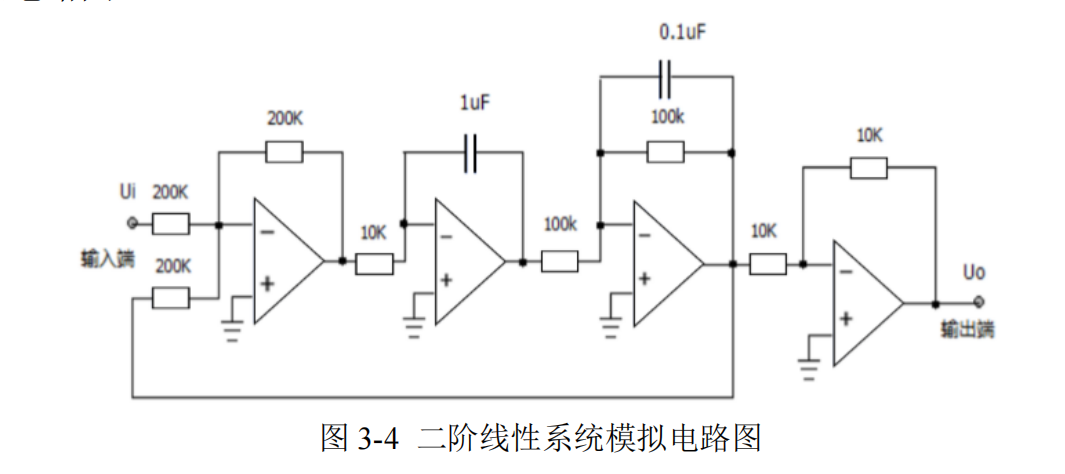
\includegraphics[width=0.8\textwidth]{3.2.png}
    \caption{二阶线性系统模拟电路图}
    \label{fig:circuit2}
\end{figure}

\subsubsection{二阶系统实测幅频特性图}
\begin{figure}[H]
    \centering
    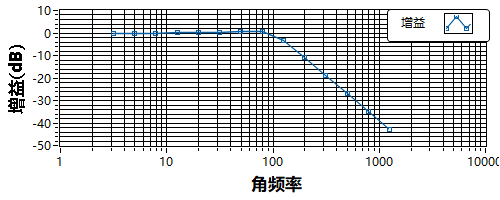
\includegraphics[width=0.8\textwidth]{2.1.png}
    \caption{二阶线性系统实测幅频增益特性曲线}
\end{figure}

\subsubsection{二阶系统实测相频特性图}
\begin{figure}[H]
    \centering
    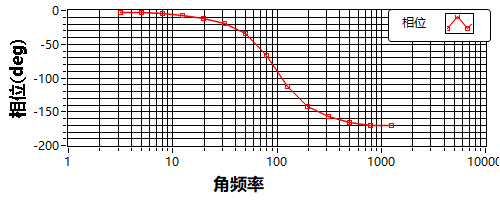
\includegraphics[width=0.8\textwidth]{2.2.png}
    \caption{二阶线性系统实测相频相位特性曲线}
\end{figure}

\subsubsection{传递函数推导}
二阶线性系统的闭环传递函数为：
\begin{equation}
\Phi(s) = \frac{K\omega_n^2}{s^2+2\zeta\omega_n s+\omega_n^2}
\end{equation}
本实验中，开环传递函数为：
\begin{equation}
G(s) = \frac{1}{0.01s(0.01s+1)}
\end{equation}
对应的闭环传递函数为：
\begin{equation}
\Phi(s) = \frac{10^4}{s^2+10^2 s+10^4}
\end{equation}
其中，自然频率 $\omega_n=100\,\mathrm{rad/s}$，阻尼比 $\zeta=0.5$，增益 $K=1$。

其频率特性为：
\begin{equation}
\Phi(\mathrm{j}\omega) = \frac{K\omega_n^2}{(\omega_n^2-\omega^2)+\mathrm{j}2\zeta\omega_n\omega}
\end{equation}
对数幅频特性：
\begin{equation}
L(\omega) = 20\lg K - 20\lg\sqrt{\bigl(1-(\omega/\omega_n)^2\bigr)^2+(2\zeta\omega/\omega_n)^2}
\end{equation}
相频特性：
\begin{equation}
\varphi(\omega) = -\arctan\left(\frac{2\zeta\omega/\omega_n}{1-(\omega/\omega_n)^2}\right)
\end{equation}

\paragraph{实验步骤}
\begin{enumerate}
    \item 求闭环传递函数表达式，确定转折频率 $\omega_n$、阻尼比 $\zeta$ 和增益 $K$ 的值。
    \item 写出线性系统的对数幅频特性 $L(\omega)$ 和相频特性 $\varphi(\omega)$ 的表达式（用 $\omega_n$、$\omega$、$\zeta$ 表示）。
    \item 计算系统的幅值和相位，角频率取值如表\ref{tab:second-order}所示，结果填入表中，并通过实验验证，分析实验数值和理论数值是否匹配。
    \item 通过实测曲线，观察二阶线性系统频率和相位，附上图形及数据。
\end{enumerate}

\subsubsection{线性系统幅频和相频理论与实测结果对比}
\begin{table}[H]
\centering
\caption{线性系统幅频和相频理论与实测结果对比}
\label{tab:second-order}
\adjustbox{max width=\linewidth}{
\begin{tabular}{|c|c|c|c|c|c|}
\hline
\multirow{2}{*}{\textbf{$\omega_n$ (rad/s)}} & $\omega$ & $L(\omega)$ 计算 & $\varphi(\omega)$ 计算 & $L(\omega)$ 实测 & $\varphi(\omega)$ 实测 \\
\cline{2-6}
 & (rad/s) & (dB) & (deg) & (dB) & (deg) \\
\hline
\multirow{4}{*}{100}
 & 10   & 0.04   & -5.71   & -0.05 & -2.37 \\
\cline{2-6}
 & 70   & 2.69   & -36.87  & 0.69  & -66.03 \\
\cline{2-6}
 & 100  & 0.00   & -90.00  & -3.24 & -112.14 \\
\cline{2-6}
 & 1000 & -40.09 & -174.23 & -42.87 & -170.75 \\
\hline
\end{tabular}
}
\end{table}

\subsection{自主设计实验}
采用实验二（典型环节的时域响应和稳定性分析）模块，设计不同阻尼比的二阶闭环系统，观察实验曲线，比较谐振频率和谐振峰值的变化，分析实测曲线与渐近线波特图的差异。

\subsubsection{自主设计实验模拟电路}
\begin{figure}[H]
    \centering
    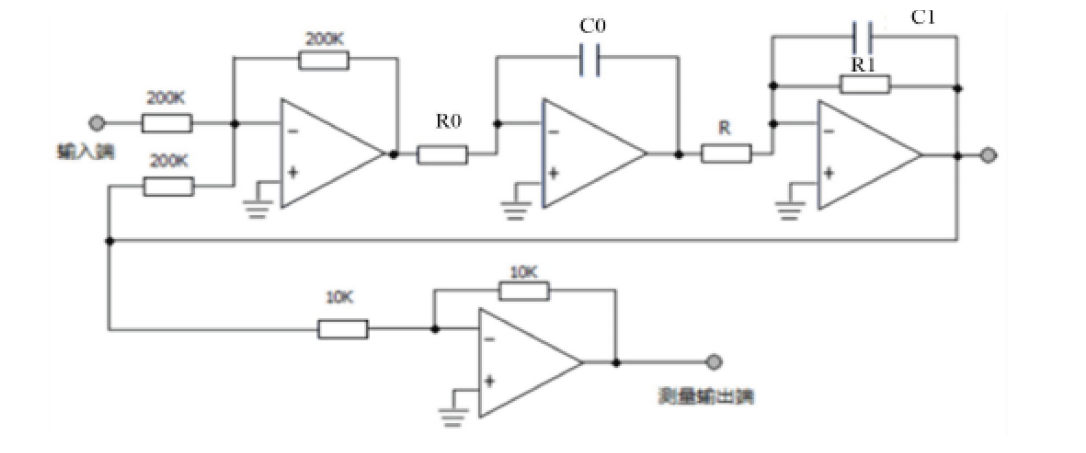
\includegraphics[width=0.8\textwidth]{3.3.png}
    \caption{自主设计实验模拟电路图}
    \label{fig:circuit3}
\end{figure}

根据图 \ref{fig:circuit3} 所示电路，该系统为典型的二阶闭环系统。本实验通过调整电路参数，设置**三组不同大小的欠阻尼阻尼比**，观察阻尼比对系统频率特性的影响。

系统的闭环传递函数模型为：
\begin{equation}
\Phi(s) = \frac{\omega_n^2}{s^2 + 2\zeta\omega_n s + \omega_n^2}
\end{equation}

\subsubsection{不同阻尼比下的实验现象分析}
本实验设置三组不同的欠阻尼阻尼比 $\zeta_1 < \zeta_2 < \zeta_3$（均满足 $\zeta<0.707$），实验现象如下：
\begin{itemize}
    \item 三组欠阻尼系统的幅频特性曲线均出现明显的谐振峰，且阻尼比越小，谐振峰值越大，谐振频率越接近系统自然频率。
    \item 阻尼比越小，相频特性曲线在谐振频率附近的变化越陡峭，系统相位变化越快。
    \item 随着阻尼比增大，谐振峰值逐渐减小，幅频特性曲线变得更加平缓，系统频带宽度略有减小，响应速度有所降低。
\end{itemize}

\section{结合实验及结果图形等，回答问题}
\begin{enumerate}[label=\textbf{\arabic*.}, leftmargin=2.5em, itemsep=1em]
\item \textbf{测试频率特性实验中，输入正弦信号的幅值、频率范围应如何选取？}

输入正弦信号幅值应适中，幅值过小易受噪声干扰，幅值过大会使系统进入非线性区。频率范围应覆盖系统的低频、中频和高频，包含系统的转折频率，确保完整绘制Bode图，全面反映系统频率特性。

\item \textbf{二阶系统在不同阻尼比的情况下，其幅频和相频特性的形状有何不同？}

所有实验系统均为欠阻尼状态，幅频特性均存在谐振峰值。阻尼比越小，谐振峰值越高，谐振频率越接近自然频率，相频特性在谐振频率附近变化越陡峭；阻尼比越大，谐振峰值越小，幅频曲线越平滑。

\item \textbf{分析三阶系统开环放大倍数 $K$ 值变化如何影响剪切频率、相角裕度及其动态性能。}

$K$ 增大，剪切频率增大，系统响应变快，但相角裕度减小，稳定性变差；$K$ 减小，剪切频率减小，响应变慢，但相角裕度增大，系统更稳定。

\item \textbf{如果对象模型未知，如何通过其频率特性曲线得到传递函数？}

通过实验测得Bode图，从幅频特性渐近线的斜率、转折频率判断环节组成，由低频段确定系统型别与增益，结合相频特性验证，最终拟合得到系统传递函数。
\end{enumerate}

\end{document}